%%%%%%%%%%%%%%%%%%%%%%%%%
\section{Experiments and Results}
\begin{figure}[htb]
\begin{subfigure}[t]{0.47\columnwidth}
        \centering
    \pgfplotstableread[row sep=\\,col sep=&]{
       cases & LR & NN & EM & VEM \\
       Fashion     & 0.6027  & 0.7006  & 0.7194 &0.7472  \\
       IT    & 0.7567 & 0.7742  & 0.7829 &0.7932 \\
    }\mydata

    \begin{tikzpicture}[scale=0.5]
    \begin{axis}[
    ybar,
    bar width=.55cm,
    width=2\textwidth,
    height=1.5\textwidth,
    legend style={at={(0.67,1.2)},
       anchor=north,legend columns= 4, font = \LARGE},
    symbolic x coords={Fashion, IT},
    xtick=data,
    enlarge x limits=0.3,
    ymin=0.60,ymax=0.80,
    ylabel={Accuracy},
    yticklabel style = {font=\huge,xshift=0.5ex},
    xticklabel style = {font=\huge,yshift=0.5ex},
    ylabel style ={font = \huge},
    ymajorgrids=true
    ]
    \addplot[draw=gray,fill=gray!40!white, thick] table[x=cases,y=LR]{\mydata};
    \addplot[draw=blue,fill=blue!40!white] table[x=cases,y=NN]{\mydata};
    \addplot[draw=black,fill=black!50!white, thick] table[x=cases,y=EM]{\mydata};
    \addplot[draw=red,fill=red!40!white, thick] table[x=cases,y=VEM]{\mydata};
    \legend{LR, NN, EM, VEM}
    \end{axis}
    \end{tikzpicture}
    \vspace{-0.15in}
        \caption{Accuracy\label{fig:acc}} 
    \end{subfigure}% 
  \hfill \hskip -2.5ex %
    	\begin{subfigure}[t]{0.47\columnwidth}
        \centering
  \centering
    \pgfplotstableread[row sep=\\,col sep=&]{
       cases & LR & NN & EM & VEM \\
       Fashion     &0.2228  & 0.2154  & 0.2467 &0.4235  \\
       IT   &0.2228  & 0.2154  & 0.2467 &0.4235 \\
    }\mydata

    \begin{tikzpicture}[scale=0.5]
    \begin{axis}[
    ybar,
    bar width=.55cm,
    width=2\textwidth,
    height=1.5\textwidth,
    legend style={at={(0.67,1.2)},
       anchor=north,legend columns= 4, font = \LARGE},
    symbolic x coords={Fashion, IT},
    xtick=data,
    enlarge x limits=0.3,
    ymin=0.2,ymax=0.5,
    ylabel={AUPRC},
    yticklabel style = {font=\huge,xshift=0.5ex},
    xticklabel style = {font=\huge,yshift=0.5ex},
    ylabel style ={font = \huge},
    ymajorgrids=true
    ]
    \addplot[draw=gray,fill=gray!40!white, thick] table[x=cases,y=LR]{\mydata};
    \addplot[draw=blue,fill=blue!40!white] table[x=cases,y=NN]{\mydata};
    \addplot[draw=black,fill=black!50!white, thick] table[x=cases,y=EM]{\mydata};
    \addplot[draw=red,fill=red!40!white, thick] table[x=cases,y=VEM]{\mydata};
    \legend{LR, NN, EM, VEM}
    \end{axis}
    \end{tikzpicture}
    \vspace{-0.15in}
        \caption{AUPRC\label{fig:auprc}} 
    \end{subfigure}% 
   \caption{\sys performance} \label{fig:variants}
\end{figure}
\iar{it values to be replaced!!}

\begin{figure}[htb]\centering
	\begin{subfigure}[t]{0.47\columnwidth}
        \centering
        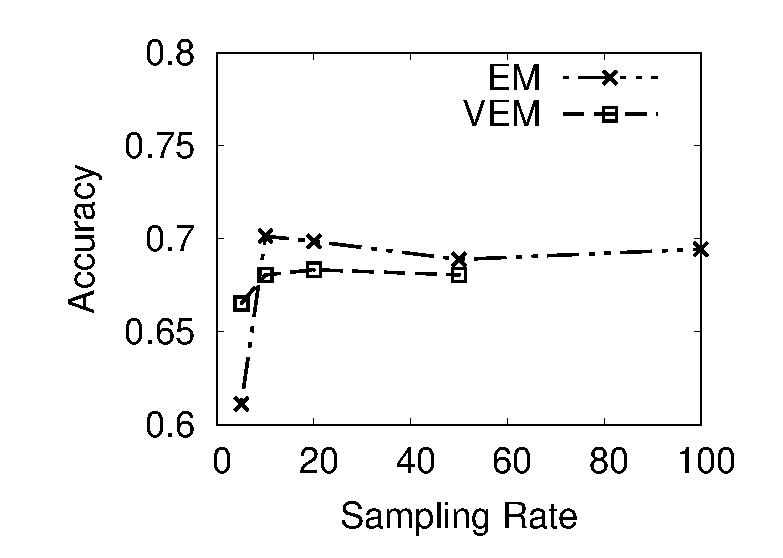
\includegraphics[width=\columnwidth]{figs/accuracy}
        \caption{Accuracy with varying sampling rate\label{fig:accuracy}} 
    \end{subfigure}% 
  \hfill \hskip -2.5ex %
    	\begin{subfigure}[t]{0.47\columnwidth}
        \centering
        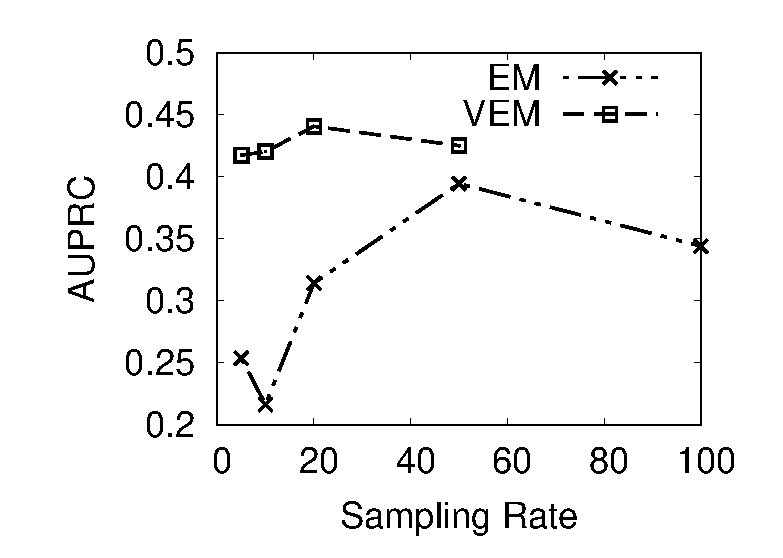
\includegraphics[width=\columnwidth]{figs/auprc}
        \caption{AUPRC with varying sampling rate\label{fig:auprc}} 
    \end{subfigure}% 
    \caption{\sys performance}
    \vspace{-5mm}
  \label{fig:sys_perf} 
\end{figure}
\iar{some values are still running!}
%%%%%%%%%%%%%%%%%%%%%%%%%